\clearpage\chapter{Radians And Degrees}
Radians. It's that pesky settings on your calculator your teacher cautions you about in class or before a test.

Up to this point, you've used degrees for everything.
\begin{itemize}
    \item All angles of triangles or intersetions between lines are in \textit{degrees}.
    \item We all learn that a right angle is exactly $90$ \textit{degrees}.
    \item We're given that a circle is $360$ \textit{degrees}.
    \item And so on...
\end{itemize}
However, as you continue moving forward in math, you'll gradually step away from degrees and use radians almost exclusively. In fact, the moment you're taught what radians are is when the switch happens. Degrees still have their place but, in my experience up to Calculus III, it's pretty much never used.

So what \textit{are} radians anyway? Like degrees, radians measure angles. But it's measured in a very specific way. For simplisity sake, I'll use the $xy$-plane to demonstrate.
\clearpage
\section{Getting Measurements}
All angle measurements begin from the positive $x$-direction, meaning the positive $x$-direction is $0$ radians. The angle increases in size as you rotate counter-clockwise. 

For example, if you wanted to get to $45$ degrees, you would begin from the positive $x$-direction (or the positive $x$-axis), and create a $45\degree$ angle between the $x$-axis and a line starting at the origin. It would look something like this:

% Text Area is 12 cm wide.
\begin{minipage}[c]{0.33\linewidth}
    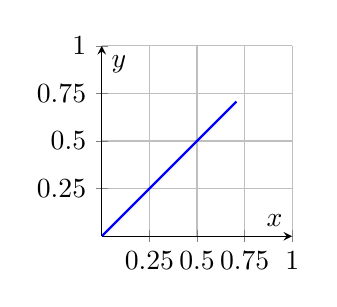
\begin{tikzpicture}
        \begin{axis}[
            axis lines = middle,
            xlabel = $x$, ylabel = {$y$},
            xmin = 0, xmax = 1,
            ymin = 0, ymax = 1,
            xtick distance={0.25}, ytick distance={0.25},
            width = 4cm,   % scale to the minipage width
            height = 4cm,
            grid = both,
            legend pos = south east,
        ]
            \addplot[blue, thick, domain=0:sqrt(2)/2, samples=100] {x};
        \end{axis}
    \end{tikzpicture}
\end{minipage}
\begin{minipage}[c]{0.66\linewidth}
    From the figure, we can see that the angle formed by the blue line and the positive $x$-axis is $45$ degrees. This also happens to be \textit{exactly} the line $y = x$. We'll get into why as we move further into the text.
\end{minipage}

If we wanted $90$ degrees, the line would instead point vertically in the positive $y$-direction like so:
\begin{center}
    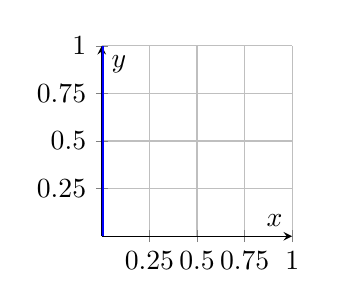
\begin{tikzpicture}
        \begin{axis}[
            axis lines = middle,
            xlabel = $x$, ylabel = {$y$},
            xmin = 0, xmax = 1,
            ymin = 0, ymax = 1,
            xtick distance={0.25}, ytick distance={0.25},
            width = 4cm,   % scale to the minipage width
            height = 4cm,
            grid = both,
            legend pos = south east,
        ]
            \draw[ultra thick, blue] (0,0) -- (0,1);
        \end{axis}
    \end{tikzpicture}
\end{center}